%%% Preamble
\documentclass[paper=a4, fontsize=11pt]{scrartcl}
\usepackage[T1]{fontenc}
\usepackage{fourier}

\usepackage[brazil]{babel}
\usepackage[protrusion=true,expansion=true]{microtype}	
\usepackage{amsmath,amsfonts,amsthm} % Math packages
\usepackage[pdftex]{graphicx}	
\usepackage{subcaption}
\usepackage{url}
\usepackage[small,compact]{titlesec}

\usepackage[margin=3cm]{geometry}
% showframe% <- only to show the page layout
\usepackage{natbib}
%%% Custom sectioning
\usepackage{sectsty}
\allsectionsfont{\centering \normalfont\scshape}

%%% Custom headers/footers (fancyhdr package)
\usepackage{fancyhdr}
\pagestyle{fancyplain}

\fancyfoot[L]{IPEA - DISET}											% Empty
\fancyfoot[C]{\projectname}											% Empty
\fancyfoot[R]{\thepage}									% Pagenumbering
\renewcommand{\headrulewidth}{0pt}			% Remove header underlines
\renewcommand{\footrulewidth}{0pt}				% Remove footer underlines
\setlength{\headheight}{13.6pt}


%%% Equation and float numbering
\numberwithin{equation}{section}		% Equationnumbering: section.eq#
\numberwithin{figure}{section}			% Figurenumbering: section.fig#
\numberwithin{table}{section}				% Tablenumbering: section.tab#


%%% Maketitle metadata
\newcommand{\horrule}[1]{\rule{\linewidth}{#1}} 	% Horizontal rule
\newcommand{\projectname}{Indicador de Tecnologias Emergentes}
\title{
		%\vspace{-1in} 	
		\usefont{OT1}{bch}{b}{n}
		\normalfont \normalsize \textsc{IPEA - DISET} \\ [25pt]
		\horrule{0.5pt} \\[0.4cm]
		\huge \projectname \\
		\horrule{2pt} \\[0.5cm]
}
\author{
		\normalfont 								\normalsize
        Fred Guth\footnote{consultor contratado.}\\[-3pt]		\normalsize
        \today
}
\date{}


%%% Begin document
\begin{document}
\maketitle
\thispagestyle{empty}
\section{Objetivo}
Antecipar tecnologias emergentes com maior potencial de impacto é essencial para um bom planejamento de políticas públicas.  Usualmente, essa atividade é bastante qualitativa, se baseando no conhecimento de especialistas e na análise de patentes e artigos científicos. Entretanto, redes sociais passaram a expressar, em tempo real, a opinião de diferentes agentes econômicos, incluindo empresas, institutos de pesquisa e publicações de especializadas em tecnologias emergentes; tornando possível mensurar quantitativamente, pelo número de menções, o julgamento agregado dessa multidão de agentes  do potencial de tecnologias (assumindo-se que os agentes mencionam mais as tecnologias em que mais vêem potencial). É um fenômeno bem relatado \citep{surowiecki2004wisdom} que julgamentos agregados deste tipo produzem boas previsões.

Neste projeto, usamos processamento de linguagem natural para criar um indicador quantitativo para tecnologias emergentes mencionadas no Twitter por contas previamente selecionadas.

\section{Metodologia}
O processo de construção do \textbf{Indicador de Tecnologias Emergentes (ITE)} abrange as seguintes etapas:
\begin{enumerate}
	\item Captura dos tweets\footnote{A curadoria das contas e a captura dos \emph{tweets} foram realizadas previamente e fogem do escopo do presente projeto.}
	\item Análise exploratória dos dados
	\item Limpeza dos dados e definição dos tópicos
	\item Construção da matriz de frequências Semestre-Tópico
	\item Detecção estatística de anomalias
	\item Geração do Indicador
\end{enumerate}
\subsection{Análise exploratória dos dados}
A análise exploratória de dados (AED) é uma abordagem de análise com objetivo de capturar um panorama geral dos dados com métodos visuais. No presente projeto, a AED não foi estensiva, até mesmo porque a maior variabilidade dos dados está no texto dos tweets o que não é capturado pela mesma. Entretanto, a AED foi importante para identificar potenciais problemas com diferentes abordagens estatísticas. Os resultados da AED serão apresentados na seção \ref{sec:dados}.
\subsection{Limpeza dos dados e definição dos tópicos}
\subsubsection{Limpeza}
A limpeza dos dados tem como objetivo padronização e a remoção de termos anômalos indesejados na análise. Todas as ações de limpeza são opcionais e podem ser \emph{desligadas} a partir de um arquivo de configuração (ver \ref{sec:config}).
\begin{itemize}
	\item  remoção de acentos
	\item  remoção de \emph{hashtags} e menções a contas do twitter: apesar de hashtags serem um sinal forte de importância no Twitter, achamos importante dar a opção de fazer a análise sem hashtags.
	\item  remoção de URLs
	\item  remoção de números: apenas palavras contendo apenas números, por exemplo "2017" é removido, enquanto "23andme" não é.
\end{itemize}
\subsubsection{Definição dos tópicos}
Qualquer palavra usada em um \emph{tweet} do corpus é, inicialmente, considerada um tópico, uma vez que, a priori, não temos como saber que uma palavra se trata de tecnologia. Pior do que isso, como analisamos também bi-gramas, combinações de duas palavras, no limite o número de tópicos pode ser quadrático em relação ao tamanho do vocabulário do corpus.

Tendo em vista que nosso corpus contém apenas mensagens curtas, o contexto em que termos tecnológicos aparecem não são muito identificáveis. Em outras palavras, queremos encontrar um pequeno sinal em um grande mar de ruído. Essa característica do problema nos leva a focar primeiro em identificar anomalias em geral, que podem ou não ser tecnológicas, deixando o problema da categorização dos tópicos como secundário.

Um primeiro passo é, então, reduzir o tamanho do vocabulário considerado. Parte disso é feito pela própria limpeza, mas consideramos também que palavras devem ter um número mínimo de menções-dia\footnote{menção-dia é frequencia de menções em diferentes dias, ou seja, várias menções no mesmo dia contam como uma.}. Além desses filtros, também estabelecemos um limite (\emph{dict\_size}) no tamanho do dicionário, pegando apenas as \emph{dict\_size} palavras com mais menções-dia no corpus.

Também filtramos \emph{stop words}, que são palavras comuns. Todas as principais bibliotecas de NLP possuem uma lista de \emph{stop words} do idioma inglês. Utilizamos a lista da biblioteca NLTK \citep{nltk} e adicionamos uma lista própria de \emph{stop words} que pode ser alterada no arquivo de configuração. Tal lista foi criada especificamente para o desafio deste projeto e parte da constatação que mesmo contas especializadas engajam-se em assuntos da cultura e capturam o zeitgeist ao longo do tempo.

\subsection{Matriz de frequências Semestre-Tópico}
\subsection{Detecção estatística de anomalias}
\subsection{Geração do Indicador}
\section{Dados}\label{sec:dados}
Lorem ipsum dolor sit amet, consectetuer adipiscing elit. Aenean commodo ligula eget dolor. Aenean massa. Cum sociis natoque penatibus et magnis dis parturient montes, nascetur ridiculus mus. Donec quam felis, ultricies nec, pellentesque eu, pretium quis, sem. In enim justo, rhoncus ut, imperdiet a, venenatis vitae, justo. Nullam dictum felis eu pede mollis pretium. Integer tincidunt. 
\begin{figure}[!h]
  \centering
  \begin{minipage}[t]{0.4\textwidth}
		\caption{Tweets por fonte.}
    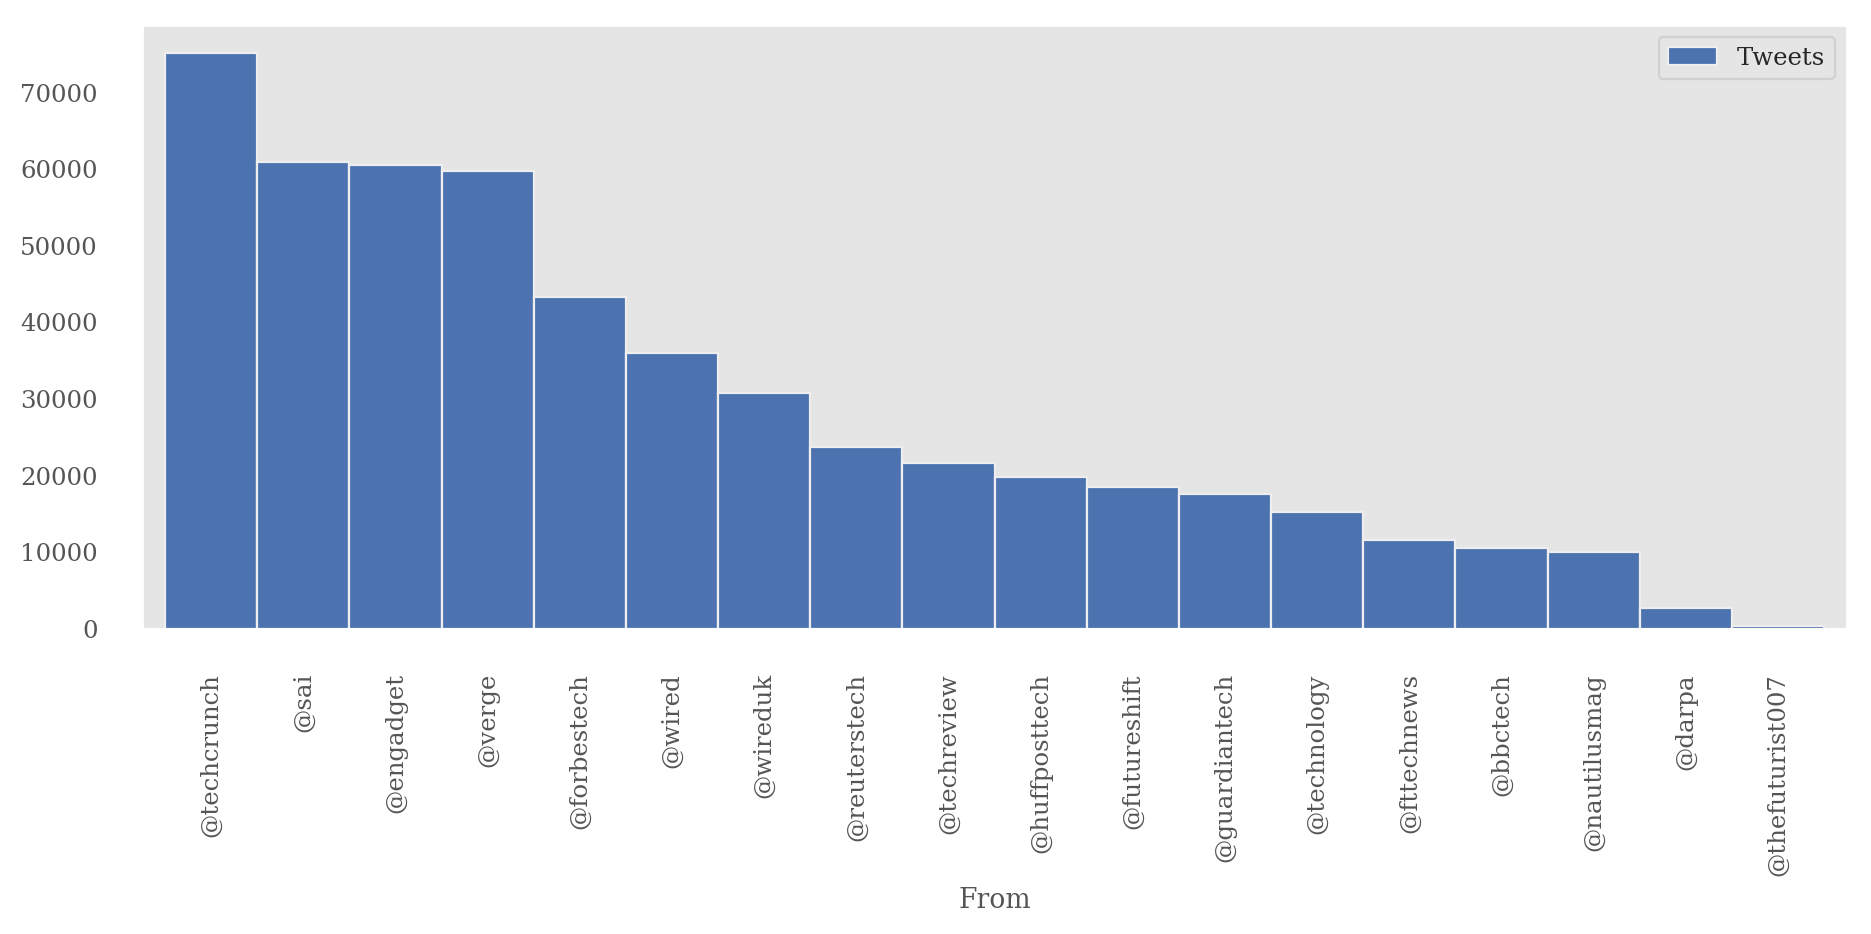
\includegraphics[width=\textwidth]{from}
  \end{minipage}
  \hfill
  \begin{minipage}[t]{0.4\textwidth}
		\caption{Tweets por dia.}
    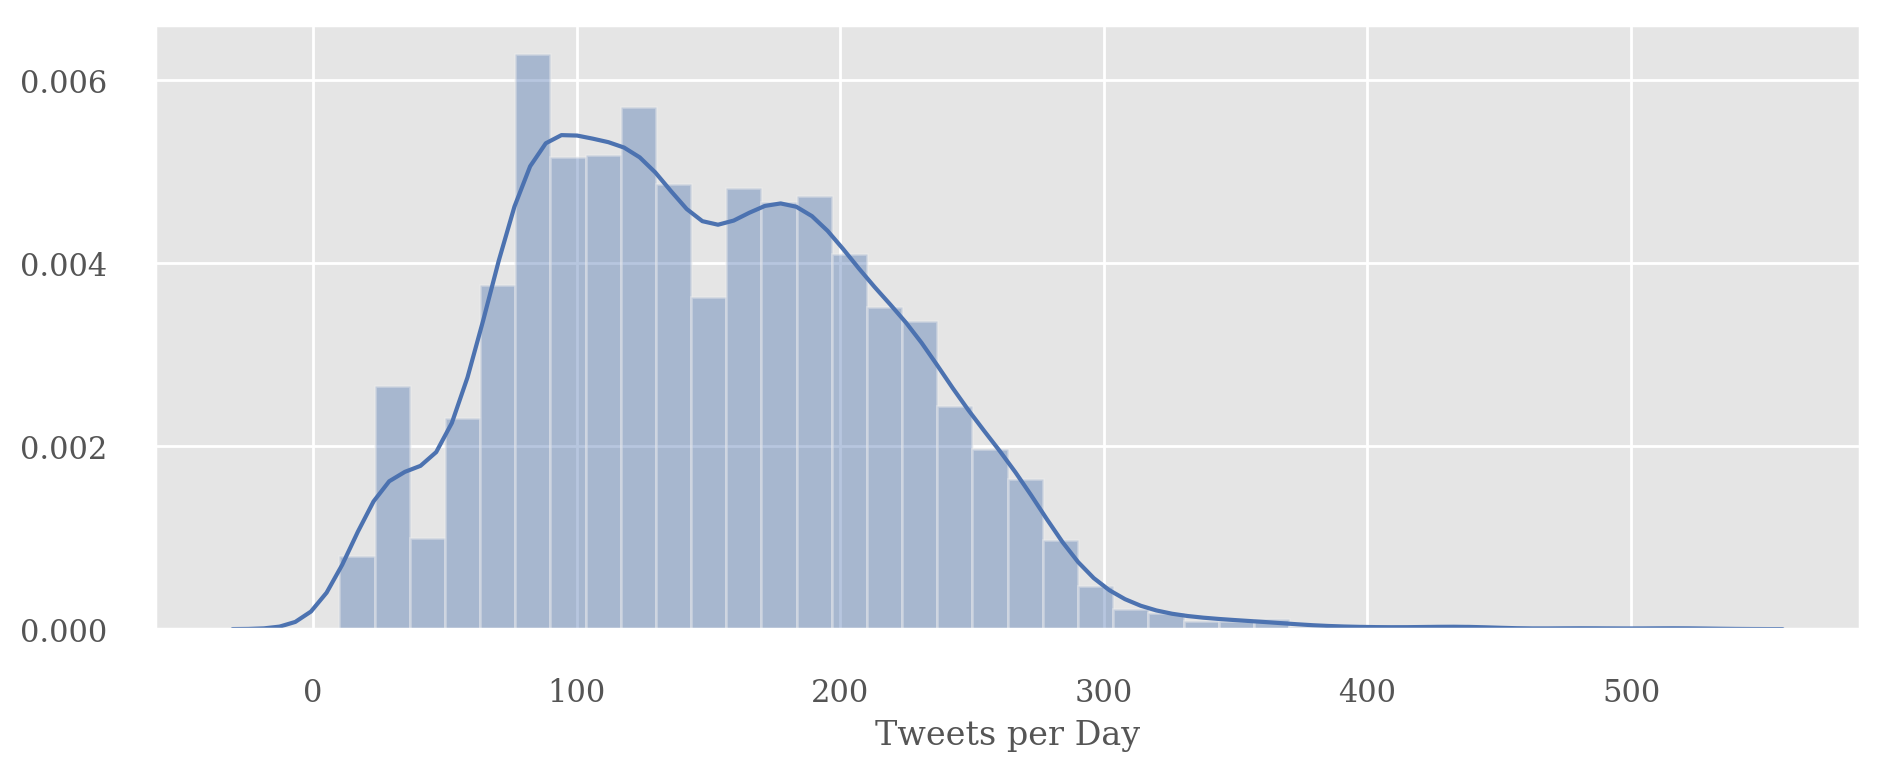
\includegraphics[width=\textwidth]{perDay}
  \end{minipage}
\end{figure}
\begin{figure}[h]
	\centering
	\caption{Tweets por período.}
	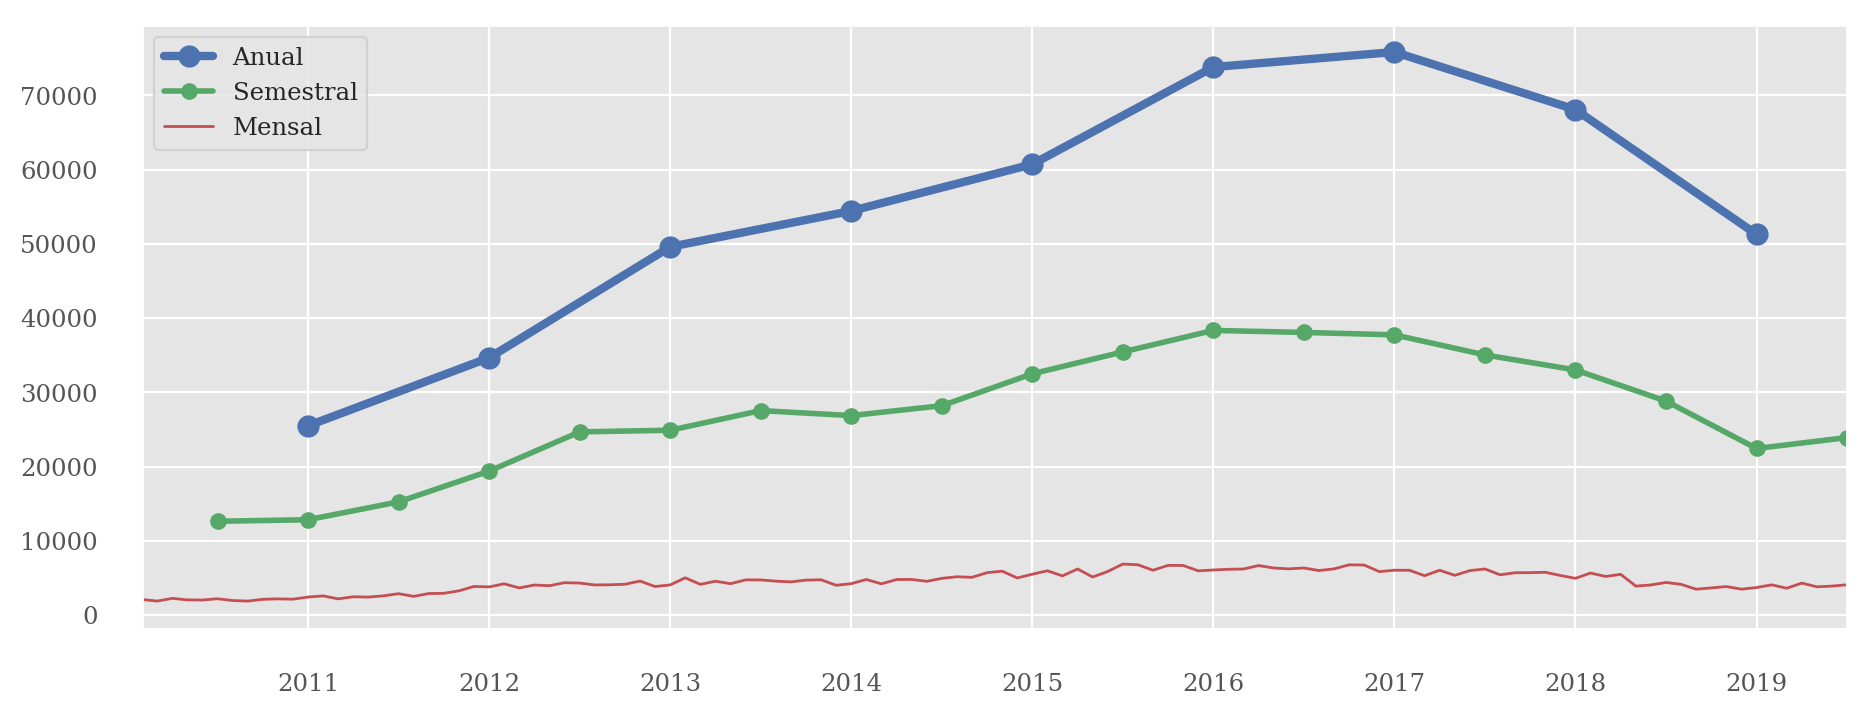
\includegraphics[width=.8\columnwidth]{anual-semestral}
	\label{fig:volume-tweets}
\end{figure}
\section{Código}
Lorem ipsum dolor sit amet, consectetuer adipiscing elit. Aenean commodo ligula eget dolor. Aenean massa. Cum sociis natoque penatibus et magnis dis parturient montes, nascetur ridiculus mus. Donec quam felis, ultricies nec, pellentesque eu, pretium quis, sem. In enim justo, rhoncus ut, imperdiet a, venenatis vitae, justo. Nullam dictum felis eu pede mollis pretium. Integer tincidunt. Cras dapibus. Vivamus elementum semper nisi. Aliquam lorem ante, dapibus in, viverra quis, feugiat a, tellus:

Phasellus viverra nulla ut metus varius laoreet. Quisque rutrum. Aenean imperdiet. Etiam ultricies nisi vel augue. Curabitur ullamcorper ultricies 

\subsection{Heading on level 2 (subsection)}
Lorem ipsum dolor sit amet, consectetuer adipiscing elit. 
\begin{align}
\end{align}
Aenean commodo ligula eget dolor. Aenean massa. Cum sociis natoque penatibus et magnis dis parturient montes, nascetur ridiculus mus. Donec quam felis, ultricies nec, pellentesque eu, pretium quis, sem.

\subsubsection{Heading on level 3 (subsubsection)}
Nulla consequat massa quis enim. Donec pede justo, fringilla vel, aliquet nec, vulputate eget, arcu. In enim justo, rhoncus ut, imperdiet a, venenatis vitae, justo. Nullam dictum felis eu pede mollis pretium. Integer tincidunt. Cras dapibus. Vivamus elementum semper nisi. Aenean vulputate eleifend tellus. Aenean leo ligula, porttitor eu, consequat vitae, eleifend ac, enim.

\paragraph{Heading on level 4 (paragraph)}
Lorem ipsum dolor sit amet, consectetuer adipiscing elit. Aenean commodo ligula eget dolor. Aenean massa. Cum sociis natoque penatibus et magnis dis parturient montes, nascetur ridiculus mus. Donec quam felis, ultricies nec, pellentesque eu, pretium quis, sem. Nulla consequat massa quis enim. 


\section{Produto}

\subsection{Example for list (3*itemize)}
\begin{itemize}
	\item First item in a list 
		\begin{itemize}
		\item First item in a list 
			\begin{itemize}
			\item First item in a list 
			\item Second item in a list 
			\end{itemize}
		\item Second item in a list 
		\end{itemize}
	\item Second item in a list 
\end{itemize}

\subsection{Example for list (enumerate)}
\begin{enumerate}
	\item First item in a list 
	\item Second item in a list 
	\item Third item in a list
\end{enumerate}
\bibliography{references.bib}
\bibliographystyle{chicago}
%%% End document
\end{document}